\documentclass[a4paper, 12pt]{article}
\usepackage[a4paper, left=30mm, right=30mm, top=30mm, bottom=30mm, marginpar=25mm]{geometry}
\usepackage{indentfirst}
\usepackage{float}
\usepackage{graphicx}
\usepackage{amsmath}
\usepackage{amsfonts}
\usepackage{amssymb}
\usepackage{geometry}
\usepackage{listings}
\usepackage{xcolor}
\usepackage{fancyhdr}
\usepackage{lastpage}
\usepackage[normalem]{ulem} 
\pagestyle{fancy}
\setlength{\headheight}{29.5pt}
\definecolor{codegreen}{rgb}{0,0.6,0}
\definecolor{codegray}{rgb}{0.5,0.5,0.5}
\definecolor{codepurple}{rgb}{0.58,0,0.82}
\definecolor{backcolour}{rgb}{0.95,0.95,0.92}
\lstset{
    backgroundcolor=\color{backcolour},   
    commentstyle=\color{codegreen},
    keywordstyle=\color{blue},
    numberstyle=\tiny\color{codegray},
    stringstyle=\color{codepurple},
    basicstyle=\ttfamily\footnotesize,
    breakatwhitespace=false,         
    breaklines=true,                 
    captionpos=b,                    
    keepspaces=true,                 
    numbers=left,                    
    numbersep=5pt,                  
    showspaces=false,                
    showstringspaces=false,
    showtabs=false,                  
    tabsize=2
}
\usepackage{pgfplots}
\pgfplotsset{compat=1.18}
\usepackage{tikz}
\usepackage{adjustbox}
\usepackage{tikz}
\usepackage{booktabs}
\renewcommand{\contentsname}{Índice}

\renewcommand*{\maketitle}{
\thispagestyle{plain}
\begin{center}
    
\includegraphics[width=7cm]{Logo-fiuba.png} 
    \\[1cm]
    \textsc{\Large Teoría de Algoritmos}\\           
    \textsc{\small Curso Echevarria}\\[0.4cm]    
    { \huge \bfseries Trabajo Práctico 1 }\\[0.3cm]      
    \rule{\textwidth}{0.4pt} \\[0.2cm] 
    {\large \today  \\[0.5cm]}                          
    \begin{minipage}{0.6\textwidth}
    \begin{flushleft}
        \large{
        \begin{itemize}
            \item Juan Claros - 111254
            \item Yoel Gaston Arlia - 111520
            \item Guido Cuppari - 111172
            \item Josue Daniel Mamani - 111514
        \end{itemize}
        }
    \end{flushleft}
\end{minipage}

\end{center}
}

\title{x}

\begin{document}

\maketitle

\newpage

\tableofcontents

\newpage
\section{{\uline{\textbf{\textit{Problema 1}}}}}
\subsection{Enunciado y Supuestos}
\begin{itemize}
    \subsubsection{Enunciado}
    \item 
    Cualquier cadena puede ser descompuesta en secuencias de palíndromos. Por ejemplo, la 
    cadena ARACALACANA se puede descomponer de las siguientes formas: 
    ARA CALAC ANA \\
    ARA C ALA C ANA \\
    A R A CALAC A N A \\
    etc. \\
    Desarrollar un algoritmo de programación dinámica que encuentre el menor número de 
    palíndromos que forman una cadena dada. Por ejemplo, para ARACALACANA debería 
    devolver 3.
    \subsubsection{Supuestos}
    \item Se supone que el algoritmo recibe una cadena (string), con una frase, y el algoritmo buscara la mínima cantidad de palíndromos posibles que forma la cadena dada por parámetro, mediante programación dinámica.
    \item La frase, si tiene espacios o caracteres especiales, van a ser tratados como letras, ejemplo A!NEUQUEN!A, va a devolver 1, ya que se es indiferente con los caracteres y letras.
    \end{itemize}
\subsection{Diseño}
\begin{itemize}
\item La ecuación de recurrencia a la que se llego es: \(opt[i] = 1\) si \(palabra[i:]\) es palíndromo y \(opt[i] = min(opt[j+1] + 1)\) para todo j tal que \(palabra[i:j+1]\) es palíndromo.

\item Subestructura óptima: La solución óptima para el prefijo \(palabra[0:i]\) depende de las soluciones óptimas de los sufijos \(palabra[j+1:]\), que son subproblemas del problema original.

Subproblemas superpuestos: Evaluar si una subcadena es palíndromo se repite muchas veces. Por eso se usa una tabla booleana \(\texttt{es\_palindromo}[i][j]\) para memorizar los resultados.

\item Se usa memoization en 2 estructuras de datos, para guardar en un arreglo de enteros (todos infinitos positivos de base) \(opt[i]\) el mínimo numero de palíndromos para \(palabra[i:]\). Y para guardar en una matriz booleana (con todas las posiciones false de base) de n x n \(\texttt{es\_palindromo}[i][j]\) si \(palabra[i:j+1]\) es un palíndromo.

\item Las estructuras de datos utilizadas para esta resolución son una lista de enteros, y una matriz de booleanos, siendo opt la lista y es\_palíndromo la matriz.

\newpage
\subsection{Pseudocodigo}
	\begin{lstlisting}[frame=single]
FUNCION min_palindromos(palabra):
    n = largo(palabra)
    
    optimo = [float('infinito')] * (n + 1)
    opt[n] = 0

    es_palindromo = [[False] * n for _ in range(n)]

    Para i desde n - 1 hasta 0 con paso -1 hacer
        Para j desde i hasta n - 1 hacer
            Si palabra[i] = palabra[j] y (j - i <= 1 o es_palindromo[i + 1][j - 1]) entonces
                es_palindromo[i][j] <- Verdadero
            FinSi
        FinPara
    FinPara

    Para i desde n - 1 hasta 0 con paso -1 hacer
        Para j desde i hasta n - 1 hacer
            Si es_palindromo[i][j] entonces
                opt[i] <- minimo entre opt[i] y (1 + opt[j + 1])
            FinSi
        FinPara
    FinPara


    DEVOLVER opt[0]

cadena = "ALLAERRESAGASRADAR"
print(min_palindromos(cadena))
	\end{lstlisting}

\end{itemize}

\newpage
\subsection{Análisis de Complejidad}
\begin{itemize}
    \item Los puntos clave para analizar la complejidad de este algoritmo son los 2 for anidados que hay tanto para el procesamiento de los palíndromos que se ejecuta para cada par i,j en:
    
	\begin{lstlisting}[frame=single]
    for i in range(n - 1, -1, -1):
        for j in range(i, n):
            if palabra[i] == palabra[j] and (j - i <= 1 or es_palindromo[i + 1][j - 1]):
                es_palindromo[i][j] = True
	\end{lstlisting}

    Y para la construcción de la tabla booleana opt[i][j] que también revisa cada subcadena \(palabra[i:j+1]\), y si la misma es palíndromo realiza una operación constante en: 
    \begin{lstlisting}[frame=single]
    for i in range(n - 1, -1, -1):
        for j in range(i, n):
            if es_palindromo[i][j]:
                opt[i] = min(opt[i], 1 + opt[j + 1])
	\end{lstlisting}

    Por lo tanto, en ambos for anidados, el peor caso implica una doble iteración sobre n, por ende la complejidad temporal total del algoritmo es de \(O(N^2)\), siendo N el largo de la cadena. 

\end{itemize}

\newpage
\subsection{Seguimiento}
\begin{itemize}
\item Vamos a hacer el seguimiento para el caso de la cadena "ARACALACANA": lo primero que hace el algoritmo es obtener el largo de la cadena recibida mediante len(), normalizar todo a mayúsculas y procede a generar las 2 estructuras utilizadas, la lista de enteros y la matriz de booleanos, para luego llegar a la primer parte importante, el preprocesamiento de los , donde se marca como True toda subcadena de \(palabra[i:j+1]\) que sea un palíndromo.

    \subitem $n = \text{largo}(\text{palabra}) = 11$
        \subitem \texttt{opt = [inf, inf, ..., inf, 0]} (longitud 12)
        \subitem \texttt{es\_palindromo[i][j] = False} para toda $i, j$

\item Para ver si un substring es palíndromo o no, se utilizan 3 factores, si palabra[i] = palabra[j] (la palabra empieza y termina con la misma letra) y si \(j - i  <= 1\) (es de 1 o 2 caracteres) o \(\texttt{es\_palindromo}[i+1][j-1]\) = True. Entonces empieza desde i = 10 y siempre lo primero que llena en cada i es la diagonal, que es trivialmente un palíndromo, al ser un solo carácter, pero empieza llenando la matriz desde el final.

\item La primer posición analizada es [10][10], siendo la cadena "A", que es un caso trivial, cumpliendo la condición y llenando la tabla en esa posición con True, luego sigue [9][9], que ocurre lo mismo que en el caso anterior, siendo simplemente el carácter "N", [9][10] no cumple la condición, ya que no empieza y termina con la misma letra, quedándose en False..., saltamos al ejemplo del siguiente palíndromo no trivial, que es [8][10] la cadena "ANA" cumple que empieza y termina con la misma letra, no tiene menos de 2 caracteres, pero \(\texttt{es\_palindromo}[i+1][j-1]\) que en este caso es [9][9] es True, entonces rellena True dándola como palíndromo.

\item Para el final de las iteraciones el algoritmo rellena la tabla ubicando True en todos los palíndromos que encuentra.

\begin{figure}[H]
    \centering
    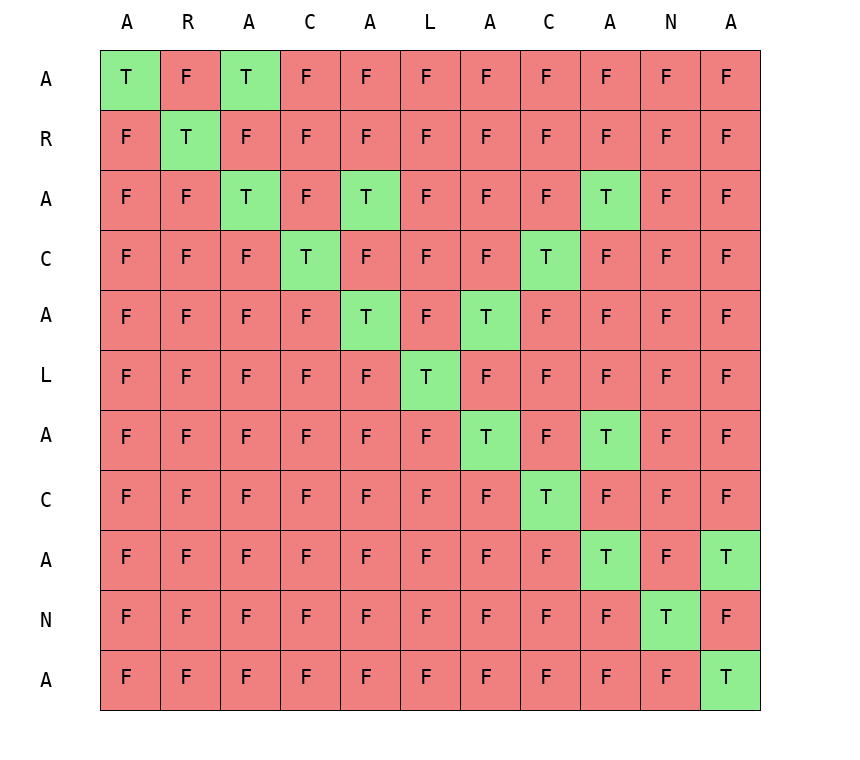
\includegraphics[width=\textwidth]{matriz_palindromos_ARACALACANA.png}
    \caption{Representación de la matriz de palíndromos.}
    \label{fig:matriz_palindromos_ARACALACANA.png}
\end{figure}


\item Una vez rellenada la tabla, pasa a la construcción de opt[i] buscando la mínima cantidad de palíndromos de la palabra, donde opt[n] = 0, siendo el caso base la string vacía, luego empieza la iteración desde i = 10 hasta 0.

\item Entonces empieza con [10][10], le pregunta a la tabla si es palíndromo, en este caso lo es, por ende opt[i] es igual al mínimo entre si mismo, que de base es infinito, y 1 + opt[j+1], que en este caso es 1 + opt[11] (que es 0), entonces opt[10] = 1. Sigue con i = 9, j = 9, se le pregunta si la [9][9] es True, lo cual es correcto, entonces se usa la ecuación siendo opt[9] = min(opt[9], 1 + opt[10], que termina siendo opt[9] = min(infinito, 2), opt[9] = 2, y así sigue con toda la tabla para finalmente encontrar el optimo que es 3.

\end{itemize}

\newpage
\subsection{Casos de prueba y mediciones}
\begin{tabular}{@{}lcc@{}}
\toprule
Entrada & Cantidad de palíndromos & Tiempo (ms) \\
\midrule
radaroso              & 2  & 0.077725 \\
123456789             & 9  & 0.077863 \\
amor a roma           & 1  & 0.108240 \\
JuanJoseGuidoYoel     & 15 & 0.162336 \\
ppppppppppppppppppp      & 1  & 0.439882 \\
anilinareconocersalas & 3  & 0.304222 \\
\bottomrule
\end{tabular}
\subsection{Resultados}
\section*{Tiempo de ejecución vs longitud de la cadena (N)}

\begin{center}
\begin{tikzpicture}
\begin{axis}[
    width=14cm,
    height=9cm,
    xlabel={Longitud de la cadena (N)},
    ylabel={Tiempo de ejecución (ms)},
    grid=major,
    enlargelimits=0.1,
    title={Relación entre longitud N y tiempo de ejecución},
    ymin=0, ymax=0.5
]

% Coordenadas con nombres como etiquetas
\addplot[
    color=blue,
    mark=*,
    thick
] coordinates {
    (8,0.077725)
    (9,0.077863)
    (10,0.108240)
    (18,0.162336)
    (20,0.439882)
    (21,0.304222)
};

% Etiquetas manuales
\node at (axis cs:8,0.077725) [above left, font=\tiny] {radaroso};
\node at (axis cs:9,0.077863) [above right, font=\tiny] {123456789};
\node at (axis cs:10,0.108240) [above left, font=\tiny] {amor a roma};
\node at (axis cs:18,0.162336) [above right, font=\tiny] {JuanJoseGuidoYoel};
\node at (axis cs:20,0.439882) [below, font=\tiny] {pppppppppppppppppppp};
\node at (axis cs:21,0.304222) [above right, font=\tiny] {anilinareconocersalas};

\end{axis}
\end{tikzpicture}
\end{center}
\section*{Curva de \(N^2\)}

\begin{center}
\begin{tikzpicture}
\begin{axis}[
    width=12cm,
    height=8cm,
    xlabel={N},
    ylabel={\(N^2\)},
    grid=major,
    domain=0:25,
    samples=100,
    title={Gráfico de \(N^2\)},
    thick
]
\addplot[
    color=blue,
    no markers
]
{x^2};
\end{axis}
\end{tikzpicture}
\end{center}

\subsection{Conclusiones}
\begin{itemize}
    \item Se ve que los sets cumplen con la complejidad prevista, exceptuando el caso de las p, donde se deja ver que las operaciones descartadas por ser menores a N\^2 afectan a la complejidad, exceptuando este caso, se ve que a medida que aumenta el largo, el tiempo sube exponencialmente, cumpliendo lo previsto.
\end{itemize}
\subsection{Generación de sets}
\begin{itemize}
    \item Los sets fueron generados arbitrariamente, para poder probar casos como distinción entre minúscula y mayúscula, espacios, ningún palíndromo, palindromos encadenados, y una cadena de un solo carácter.
\end{itemize}

\section{{\uline{\textbf{\textit{Problema 2}}}}}
\subsection{Supuestos}
    Concesiones Argentina 2000 SRL tiene la concesión de los espacios publicitarios en las 
paradas de colectivos de un municipio. Son en total 200 paradas y tiene ofertas de distintos 
productos para el próximo mes: 
\begin{itemize}
    \item Cliente A ofrece USD 50000 por ocupar 30 paradas 
    \item Cliente B ofrece USD 100000 por ocupar 80 paradas o USD 120000 por 120 
    paradas (sólo una de ambas opciones) 
    \item Cliente C ofrece USD 100000 por ocupar 75 paradas 
    \item Cliente D ofrece USD 80000 por ocupar 50 paradas 
    \item Cliente E ofrece USD 5000 por ocupar 2 paradas 
    \item Cliente F ofrece USD 40000 por ocupar 20 paradas 
    \item Cliente G ofrece USD 90000 por ocupar 100 paradas 
\end{itemize}

    Por ser competidores directos, no se puede hacer publicidad simultáneamente de los 
clientes A y D. Se desea determinar a qué clientes se concesionará la publicidad de las 
paradas para maximizar el beneficio total. 

\subsection{Variables}
    las variables para resolver el problema son las siguientes:
\begin{itemize}
    \item a = incluir cliente A (variable binaria)
    \item $b_1$ = incluir cliente B de 80 paradas (variable binaria)
    \item $b_2$ = incluir cliente B de 120 paradas (variable binaria)
    \item c = incluir cliente C (variable binaria)
    \item d = incluir cliente D (variable binaria)
    \item e = incluir cliente e (variable binaria)
    \item f = incluir cliente f (variable binaria)
    \item g = incluir cliente G (variable binaria)
\end{itemize}

\subsection{Modelo de programacion lineal}
    La funcion objetivo a maximizar es la siguiente:
\begin{align*}
    z &= 50000a + 100000b_1 + 120000b_2 + 100000c + 80000d + 5000e + 40000f + 90000g \\
    \max(z)
\end{align*}

Restricciones del modelo:
\begin{align*}
    30a + 80b_1 + 120b_2 + 75c + 50d + 2e + 20f + 100g &\leq 200 \\
    b_1 + b_2 &\leq 1 \\
    a + d &\leq 1
\end{align*}
\begin{itemize}
    \item La primera ecuacion nos indica el total de paradas de se concesionara a los clientes para la publicidad no supere las 200 paradas disponibles.
    \item La segunda ecuacion nos indica que de las ambas opciones que tiene el cliente B solo pueda ser 1 y no las 2.
    \item La tercera ecuacion nos indica que que no se puede hacer publicidad simultaneamente de los cliente A y D.
    
\end{itemize}

\subsection{Solucion}
    Para resover el modelo se desarrollo un programa utilizando python y pulp, el cual es el siguinte:
    \begin{figure}[H] 
		\centering
		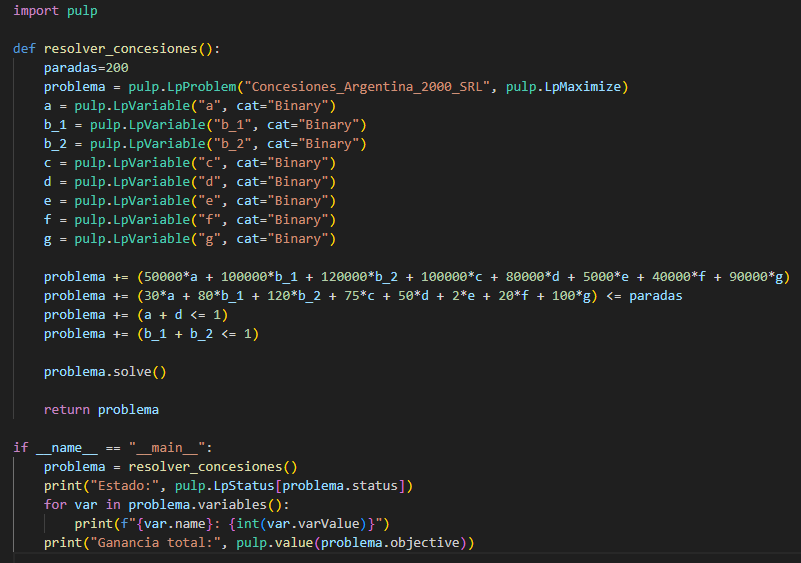
\includegraphics[width=\textwidth]{modelo.png}
	\end{figure}

    como resultado dio que para maximizar la ganancia tendriamos que escoger a los clientes A, B(la opcion de 80 paradas), c y e.

\subsection{Informe}
    La solucion del modelo de programacion lineal nos propone que para determinar a qué clientes se concesionará la publicidad de las paradas para maximizar el beneficio total son las siguientes:
\begin{itemize}
    \item Cliente A ofrece USD 50000 por ocupar 30 paradas 
    \item Cliente B ofrece USD 100000 por ocupar 80 paradas
    \item Cliente C ofrece USD 100000 por ocupar 75 paradas 
    \item Cliente E ofrece USD 5000 por ocupar 2 paradas 
\end{itemize}
    con estos resultados nos queda una ganancia de USD 255000 y la cantidad de paradas utilizadas para la publicidad son de 187, la cantidad de paradas no llega al limite pero tampoco se puede utilizar para darles publicidad a otros clientes porque las paradas requeridas por los otros clientes es mayor a la disponible.
\end{document}